\begin{center}
	\Huge
	Normalfordelingen
\end{center}
\section*{Approksimation af binomialfordelingen}
\stepcounter{section}
Vi starter vores normalfordelingsforløb op med at betragte binomialfordelingen fra sidste år.

\begin{exa}\label{exa:bin1}
	En mønt kastes 1000 gange. Vi betragter udfaldet krone som en succes. Antallet af kroner kan så modelleres som en binomialfordelt stokastisk variabel med sandsynlighedsparameter $p = 0.5$ og
	antalsparameter $n = 1000$ skrevet $X \sim B(1000,0.5)$. Vi husker på, at sandsynlighedsfunktionen for denne binomialfordelte stokastiske variabel er
	\begin{align*}
		P(X=k) =\binom{n}{k}(p)^k(1-p)^{n-k}= \binom{1000}{k}(0.5)^k(0.5)^{1000-k}.
	\end{align*}
	Vi tegner sandsynlighedsfunktionen som et pindediagram. Dette kan ses på Fig. \ref{fig:binompinde}
	\begin{figure}[H]
		\center
		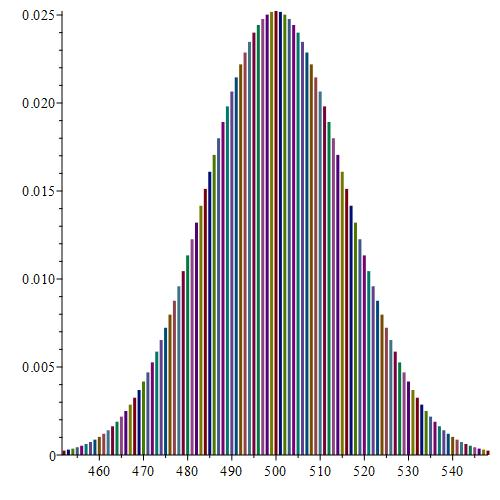
\includegraphics[width=0.7\textwidth]{Billeder/binompinde.jpg}
		\caption{Plot af sandsynlighedsfunktion for $X \sim B(n,p)$.}
		\label{fig:binompinde}
	\end{figure}
	Af Fig. \ref{fig:binompinde} kan det tydeligt ses, at det mest sandsynlige udfald er 500. 
	Vi husker på, at middelværdien $\mu$ for $X \sim B(n,p)$ er givet ved
	\begin{align*}
		\mu = np = 1000\cdot 0.5 = 500
	\end{align*}
	og spredningen $\sigma$ er givet ved
	\begin{align*}
		\sigma = \sqrt{np(1-p)} = \sqrt{1000\cdot 0.5\cdot 0.5} \approx 15.8
	\end{align*}		
\end{exa}

Den første henseende vi skal betragte normalfordelningen i er til at approksimere binomialfordelingen når $n$ bliver stor. Lad os derfor betragte den binomialfordelte stokastiske variabel fra Eksempel \ref{exa:bin1}
\begin{exa}
	Vi betragter fire forskellige binomialfordelte variable. Én hvor vi kaster 10 gange med en mønt, én hvor vi kaster 100 gange med en mønt, én hvor vi kaster 300 gange med en mønt og én hvor vi kaster 
	1000 gange med en mønt. Disse lyder henholdsvist
	\begin{align*}
		&X_1 \sim B(10,0.5), &&X_2 \sim B(100,0.5),\\
		&X_2 \sim B(300,0.5), &&X_4 \sim B(1000,0.5).
	\end{align*}
	Disse har henholdsvist middelværdierne
	\begin{align*}
		&\mu_1 = 5, &&\mu_2 = 50, \\
		&\mu_3 = 150, &&\mu_4 = 500. 
	\end{align*}
	De har desuden spredningerne
	\begin{align*}
		&\sigma_1 \approx 1.58, && \sigma_2 = 5\\
		&\sigma_3 \approx 8.66, && \sigma_4 \approx 15.81.
	\end{align*}
	Vi vil nu for hver af disse stokastiske variable approksimere dem med en normalfordelt stokastisk variabel der har samme middelværdi og spredning som de binomialfordelte stokastiske variable 
	henholdsvist. Hvad dette rent faktisk betyder vil vi præcisere senere. 
	Approksimationerne fremgår af Fig. \ref{fig:pinde4}
	\begin{figure}[H]
		\center
		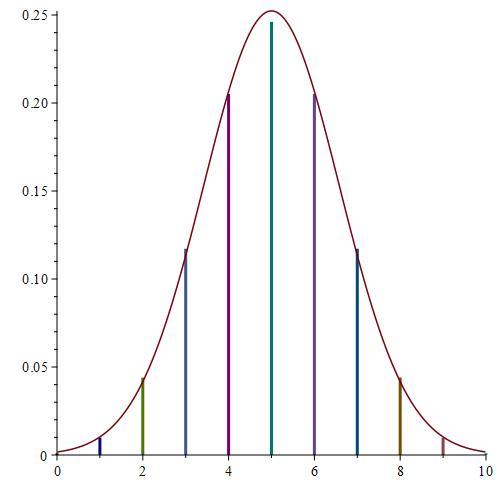
\includegraphics[width=0.45\textwidth]{Billeder/binompinde10}
		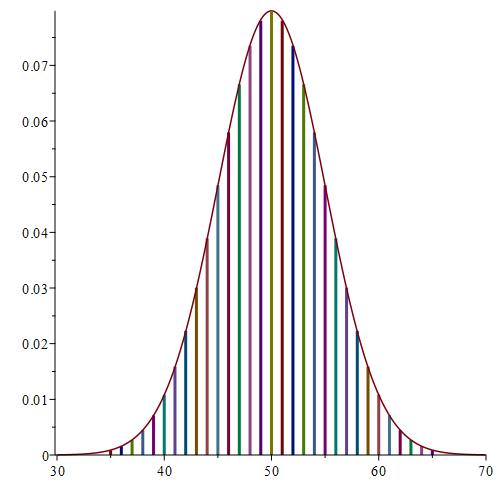
\includegraphics[width=0.45\textwidth]{Billeder/binompinde100}
		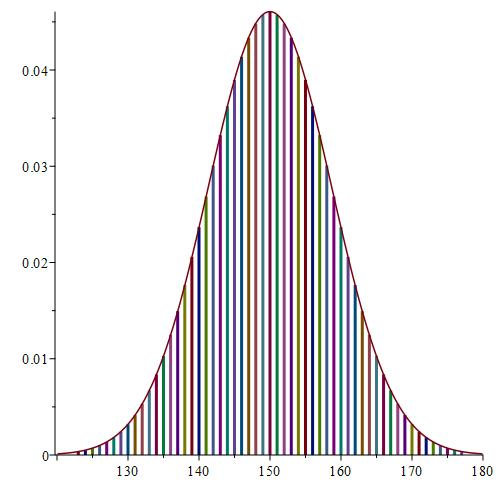
\includegraphics[width=0.45\textwidth]{Billeder/binompinde300}
		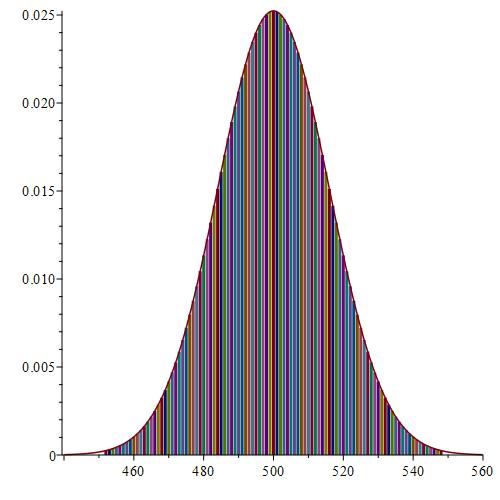
\includegraphics[width=0.45\textwidth]{Billeder/binompinde1000}
		\caption{Normalfordelingsapproksimation af binomialfordeling.}
		\label{fig:pinde4}
	\end{figure}
	Af Fig \ref{fig:pinde4} kan vi se, at approksimationen bliver bedre og bedre jo større $n$ er. Det skal også bemærkes, at approksimationen bliver dårlig, når $p$ er tæt på 0 eller 1, men den er god, 
	hvis $p = 0.5$ som i dette tilfælde. 
\end{exa}

Kurverne der approksimerer binomialfordelingerne kaldes for \textit{Gauss-kurver} og de udgør det, vi kalder for \textit{tæthedsfunktionen} for normalfordelingen. Vi definerer nu den normalfordelte stokastiske variabel.

\begin{defn}[Normalfordelt stokastisk variabel]
	Den normalfordelte stokastiske variabel $X \sim N(\mu,\sigma)$ er den kontinuerte stokastiske variabel, der har tæthedsfunktionen
	\begin{align*}
		f(x) = \frac{1}{\sigma \sqrt{2\pi}}e^{-\frac{1}{2}\left(\frac{x-\mu}{\sigma}\right)^2}
	\end{align*}
	og \textit{fordelingsfunktionen}
	\begin{align*}
		P(X\leq a) = F(a) = \int_{-\infty}^a f(x) dx.
	\end{align*}
\end{defn}
Der er en vigtig pointe her! For en kontinuert stokastisk variabel er sandsynligheden for et diskret udfald $P(X=k) = 0$, da det dækker over integralet på et interval med længde 0.

En særlig normalfordelt stokastisk variabel fås, når $\mu = 0$, og $\sigma = 1$. Så siges $X\sim N(0,1)$ at være en \textit{standardnormalfordelt stokastisk variabel}. 

\begin{exa}
	En stor undersøgelse af højden af danske kvinder har bestemt, at danske kvinders højde er approksimativt normalfordelt med middelværdi 167.1 og spredning 6.8, altså
	\begin{align*}
		X_k \sim N(167.1,6.8)
	\end{align*}
	Tilsvarende er højden af mænd normalfordelt med
	\begin{align*}
		X_m \sim N(181.4, 9.1).
  	\end{align*}	 
  	Tæthedsfunktionen og fordelingsfunktionen for disse stokastiske variable kan ses af Fig. \ref{fig:hojde}.
  	\begin{figure}[H]
  		\center
  		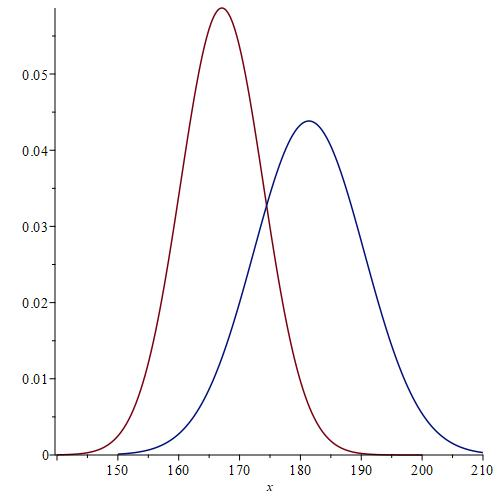
\includegraphics[width=0.45\textwidth]{Billeder/mk.jpg}
  		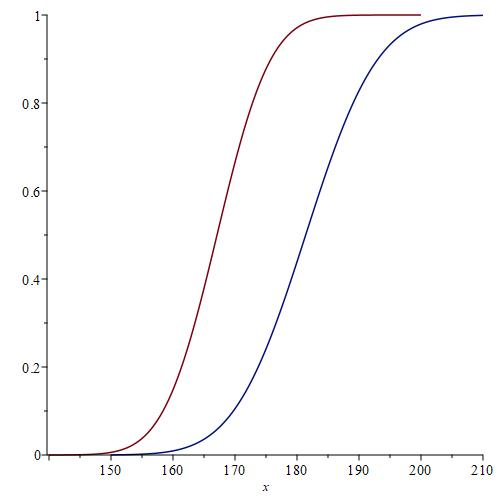
\includegraphics[width=0.45\textwidth]{Billeder/mkcdf.jpg}
  		\caption{Tæthedsfunktioner og fordelingsfunktioner henholdsvist for fordelingen af mænd og kvinders højde i Danmark. }
  		\label{fig:hojde}
  	\end{figure}
  	For den normalfordelte stokastiske variabel gælder der, at 
  	\begin{align*}
  		P(\mu - \sigma < X < \mu + \sigma) &\approx 0.683,\\
  		P(\mu - 2\sigma < X < \mu + 2\sigma) &\approx 0.954,\\
  		P(\mu - 3\sigma < X < \mu + 3\sigma) &\approx 0.997.
  	\end{align*}
  	Alle udfald med afstand to spredninger fra middelværdien kaldes for normale udfald. 
  	Alle udfald med større end tre spredningers afstand fra middelværdien kaldes for exceptionelle udfald. 
  	Tager vi udgangspunkt i højderne for kvinderne så vil vi altså have, at 
  	\begin{align*}
  		P(160.3< X < 173.9) &\approx 0.683,\\
  		P(153.5< X < 180.7) &\approx 0.954,\\
  		P(146.7 < X < 187.5) &\approx 0.997.
  	\end{align*}
  	Et exceptionelt udfald kan i dette tilfælde være en person med højden 140 centimeter. Det skal dog bemærkes, at højden kun er approksimativt normalfordelt, og bliver dårlig særligt i halerne på 
  	fordelingen. 
\end{exa}


\section*{Opgave 1}

En person slår med en terning 115 gange, og han antager, at antallet af seksere er binomialfordelt. 
\begin{enumerate}[label=\roman*)]
	\item Bestem antalsparameteren $n$ og sandsynlighedsparameteren $p$ for den binomialfordelte stokastiske variabel $X_b$, der beskriver antallet af seksere.
	\item Bestem middelværdien og spredningen for $X_b$.
	\item Bestem en normalfordelt stokastisk variabel $X_n$, der kan bruges til at approksimere $X_b$
	\item Brug fordelingsfunktionen for $X_n$ til at approksimere sandsynligheden for at få mindre end 14 seksere. (Sammenlign eventuelt med sandsynlighed fra fordelingsfunktionen for $X_b$)
\end{enumerate}

\section*{Opgave 2}
I et klinisk forsøg har et lægemiddel vist sig at helbrede $67.3\%$ af patienter, der får lægemiddelet ordineret. I et land gives lægemiddelet til 27.361 personer.
\begin{enumerate}[label=\roman*)]
	\item Bestem antalsparameteren $n$ og sandsynlighedsparameteren $p$ for den binomialfordelte stokastiske variabel $X_b$, der beskriver antallet af helbredte
	\item Bestem middelværdien og spredningen for $X_b$.
	\item Bestem en normalfordelt stokastisk variabel $X_n$, der kan bruges til at approksimere $X_b$
	\item Brug fordelingsfunktionen for $X_n$ til at approksimere sandsynligheden for at mere end $20.000$ helbredes. 
\end{enumerate}
\section*{Opgave 3}

En producent af printplader har bestilt 150.000 kondensatorer. Af disse har han fået 2377 defekte kondensatorer, hvilket han synes er lidt for mange. Producenten af kondensatorer lover, at kun $1\%$ af kondensatorerne er defekte. 
\begin{enumerate}[label=\roman*)]
	\item Bestem antalsparameteren $n$ og sandsynlighedsparameteren $p$ for den binomialfordelte stokastiske variabel $X_b$, der beskriver antallet af defekte kondensatorer, hvis 
	vi antager, at producenten af kondensatorer taler sandt. 
	\item Bestem middelværdien og spredningen for $X_b$.
	\item Bestem en normalfordelt stokastisk variabel $X_n$, der kan bruges til at approksimere $X_b$
	\item Brug fordelingsfunktionen for $X_n$ til at approksimere sandsynligheden for at få 2377 eller flere defekte kondensatorer. Har producenten af printplader grund i sin mistanke?
\end{enumerate}

\section*{Opgave 4}
I har en aflevering (: